%Dokumentinnstillinger:---------------------------------
%Ved å google flitting kan du finne ut hva de forskjellige tingene her betyr, og hvordan du kan gjøre eventuelle endringer.
\documentclass[a4paper,11pt,norsk]{article}
\usepackage[utf8]{inputenc}
\usepackage{a4wide}
\usepackage{lmodern}
\usepackage[T1]{fontenc}
\usepackage{babel}
\usepackage{textcomp}

\setlength{\parindent}{0pt} 
\setlength{\parskip}{2ex}
\usepackage{fixltx2e}
\usepackage{amsmath}
\usepackage[pdftex, pdfborderstyle={/S/U/W 0}]{hyperref}
\usepackage{graphicx}
\usepackage[font=small,labelfont=bf]{caption}
\usepackage{tabularx}
\usepackage{multirow}
\usepackage{circuitikz}
% Adds seperation between two elements with a comma. Format: "    ,    ".
\newcommand{\comma}{\quad , \quad}
% Gives double underline under selected text.
\def\dunderline#1{\underline{\underline{#1}}}
% Faster way to make an equation that can be formatted with "&" to look nice.
\def\spliteq#1{\begin{equation}\begin{split}{#1}\end{split}\end{equation}\\}
%------------------------------------- End -------------------------------------

\begin{document}

%Headingdel:---------------------------------------------
\begin{minipage}[c]{0.15\textwidth}

\includegraphics[width=2.0cm]{Design_projects/elsys_pos_staaende_ntnu.png}
\end{minipage}
\begin{minipage}[c]{0.85\textwidth}

\renewcommand{\arraystretch}{1.7}
\large 
\begin{tabularx}{\textwidth}{|X|X|}
\hline
\multicolumn{2}{|l|}{} \\
\multicolumn{2}{|l|}{\huge \textbf{Designnotat 1}} \\
\multicolumn{2}{|l|}{}  \\
\hline
\multicolumn{2}{|l|}{Tittel: 
%Skriv inn tittel her:------------------------------------------
Enkle prinsipper for støyfjerning (AC-strøm)
} \\
\hline
\multicolumn{2}{|l|}{Forfattere: 
%Skriv inn forfattere her:--------------------------------------
Sindre Danielsen
} \\
\hline
%Skriv inn versjon og dato her her:-----------------------------
Versjon: 3.0 & Dato: 09.06.21
\\
\hline 
\end{tabularx}
\end{minipage}
\normalsize

%Automatisk generert innholdsfortegnelse:------------------

\setlength{\parskip}{0ex}
\renewcommand{\baselinestretch}{0.1}\normalsize
\tableofcontents
\renewcommand{\baselinestretch}{1.00}\normalsize
\setlength{\parskip}{2ex}
\rule{\textwidth}{1pt}

%Selve rapporten:----------------------------------------÷
\newpage
\section{Problembeskrivelse}
\label{sec:innledning}
Elektrisk støy er noe som forekommer i forbindelse med signalbehandling, og ofte kan det være hensiktsmessing å fjerne det. Det ønskes da å utvikle et system vist ved figur~\ref{fig:støyfjerner}.
\begin{figure}[htbp]
    \centering
    \begin{circuitikz} [american voltages, european resistors, baseline=(current bounding box.center)]
        \ctikzset { label/align = straight }
        \draw (2.5,2)
        to[short, -o] (4,2)
        to[short] (4.5,2)
        (4, 1.6) to [open,v=$\mathbf{x(t)}$] (4,0.4)
        % Bottom-left side
        (2.5,0) to[short, -o] (4,0)
        to[short] (4.5,0)
        % Top-right side
        (8.5,2) to[short, -o] (9,2)
        to[short] (10, 2)
        (9, 1.6) to [open,v=$\mathbf{\hat{s}(t)}$] (9,0.4)
        % Bottom-right side
        (10, 0) to[short, -o] (9,0)
        to[short] (8.5,0);
        
        % Nivåregulator
        \node[draw,minimum width=4cm,minimum height=3.8cm,anchor=south west] at (4.5,-0.90){$\mathbf{H}$};

        
    \end{circuitikz}
    \caption{Støyfjerning for vekselstrøm.}
  \label{fig:støyfjerner}
\end{figure}
\\
Den tar inn et signal med støy $x(t)$ og gir oss ut et forbedret signal $\hat{s}(t)$. Funksjonen til støyfjerneren $H$ er å stoppe en unønsket frekvens ved bruk av et båndstopp filter, som blir forklart i seksjon~\ref{sec:prinsipielllosning}. \\
Ved bruk av et slikt system er kravet at kun et lite frekvensområdet skal stoppes. Samtidig skal resten av frekvensområdet skal være minimalt påvirket, som vil si amplituden på signalet.

\newpage
\section{Prinsipiell løsning}
\label{sec:prinsipielllosning}
Slik nevnt i seksjon~\ref{sec:innledning}, så kan støyfjerning løses ved bruk av et båndstopp filter. \\
En krets for et enkelt båndstoppfilter er gitt ved figur~\ref{fig:båndstoppfilter}. 
\begin{figure}[htbp]
    \centering
    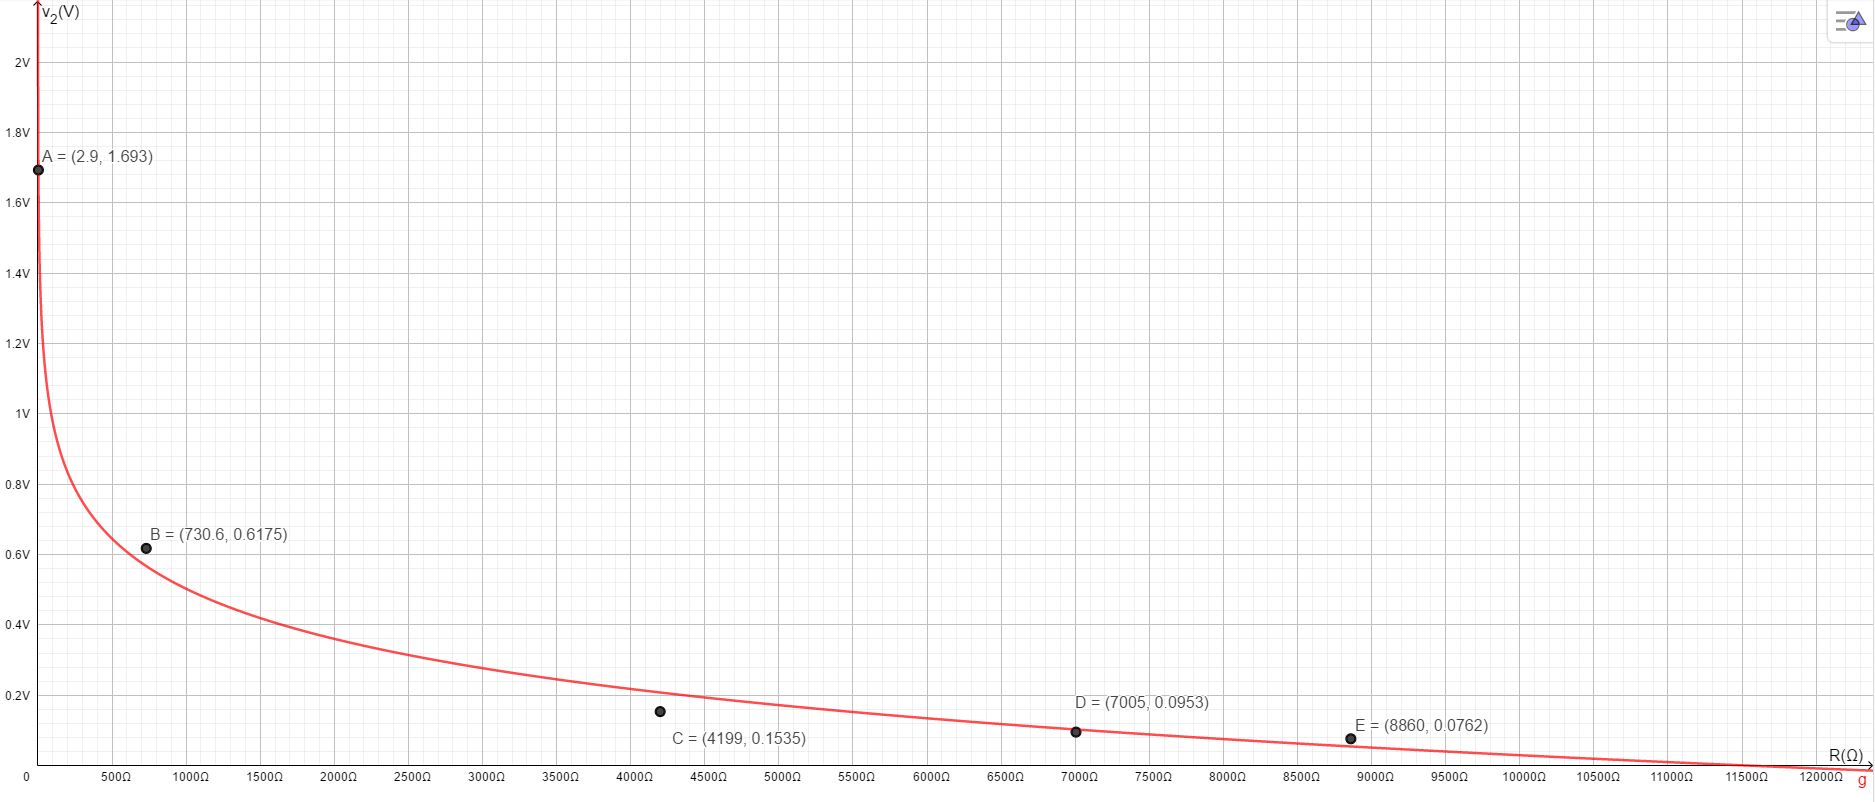
\includegraphics[width=1\textwidth]{img/graph}
    \begin{circuitikz} [american voltages, european resistors, european vresistors, baseline=(current bounding box.center)]
        \ctikzset { label/align = straight }
        \draw (0,0)
        to[short, o-] (2.5,0)
        to[R=$R_1$] (2.5, -2);
        \draw (2.5, -2)
        to[capacitor=$C_1$] (2.5, -4)
        ;
        \draw(2.5, -4)
        to[american inductor=$L_1$] (2.5, -6)
        (0, -2) to[open, v=$x_1$] (0,-4)
        (6, -3) to[open, v=$\hat{s}_1$] (6,-5)
        ;
        \draw (2.5,-2) to[short, -o](6, -2)
        ;
        \draw (0,-6) to[short, o-o] (6,-6)
        ;
        \node[draw,dashed,minimum width=3.5cm,minimum height=8cm,anchor=south west] at (1,-7);
        
        
    \end{circuitikz}
    \caption{Båndstoppfilter}
    \label{fig:båndstoppfilter}
\end{figure}
\\
Hvis inngangsignalet $x_1$ inneholder støy, så vil utgangsignalet $\hat{s}_1$ fjerne frekvensområdet ønsket ved et båndstoppfilter gitt av resonansfrekvensen $w_0$. Den er er bestemt av kondenstaoren $C_1$ og  spolen $L_1$. Størrelsen på motstanden $R_1$ vil da gi signaldempningen i området rundt resonansfrekvensen. Denne signaldempninger kan vi utlede fra totalimpedansen:
\\
$$Z = R_1 + j\omega L_1 - j \frac{1}{\omega C_1}$$
\begin{equation}
    \implies R =  Z - j\omega L_1 + j \frac{1}{\omega C_1}
\end{equation}
for $\omega \in \left<0,\infty\right> \backslash\{\omega_0\}$, der resonnansfrekvensen er gitt ved $w_0 = 2\pi f_0$.
\\
\\
Vi kaller støyets frekvens for $f_s$, slik at vi finner $C_1$ og $L_1$ ved \\ resonannsfrekvensen ($\omega_0 = 2\pi f_s$): 
    $$2\pi f_s = \frac{1}{\sqrt{C L}}$$
\begin{equation}
    \implies L = \frac{1}{C (2 \pi f_s)^2} \comma C = \frac{1}{L (2\pi f_s)^2}
\end{equation}\label{eq:resonnans}
\\
\newpage
For at området i nærheten av $w_0$ skal påvirkes minst mulig av båndstoppfilteret, så kan vi kaskadekoble flere båndstoppfilter. Dette er vist ved figur~\ref{fig:kaskadekobling}.
\begin{figure}[htbp]
    \centering
    \begin{circuitikz} [american voltages, european resistors, baseline=(current bounding box.center)]
        \ctikzset { label/align = straight }
        \draw (0,2)
        % Top-Left of H_{n-1}
        to[short, -o] (0.5,2)
        to[short] (1,2)
        % Input signal x
        (0.5, 1.6) to [open,v=$\mathbf{x(t)}$] (0.5,0.4)
        % Bottom-Left of H_{n-1}
        (0,0) to[short, -o] (0.5,0)
        to[short] (1,0)
        
        % Op-amp
        (7, 1.5) node[op amp,yscale=-1] (opamp) {}
        (opamp.+) to[short] (5, 2)
        (opamp.-) |- (6, 0.25) to[short] (8, 0.25) -| (opamp.out)
        (opamp.out) to[short,o-] (8.2, 2)
        to[short] (9.7, 2)
        
        % Under op-amp
        (9.7, 0) to[short] (5, 0)
        
        % Top-Right of H_{n}
        (13.7,2) to[short, -o] (14.2,2)
        to[short] (14.7,2)
        % Bottom-Right of H_{n}
        (13.7,0) to[short, -o] (14.2,0)
        to[short] (14.7,0)
        % Output signal
        (14.2, 1.6) to [open,v=$\mathbf{\hat{s}(t)}$] (14.2,0.4)

        % Bottom-Left of H_{n-1}
        (0,0) to[short, -o] (0.5,0)
        to[short] (1,0);
        
        % H boxes
        \node[draw,minimum width=4cm,minimum height=3.8cm,anchor=south west] at (1,-0.90){$\mathbf{H_{n-1}}$};
        \node[draw,minimum width=4cm,minimum height=3.8cm,anchor=south west] at (9.7,-0.90){$\mathbf{H_{n}}$};

        
    \end{circuitikz}
    \caption{Kaskadekobling med buffer som mellomledd.}
  \label{fig:kaskadekobling}
\end{figure}
\\
Der $H_{n-1}$ og $H_{n}$ tilsvarer båndstoppfilter nummeret. Poenget er at desto flere filter, desto mindre forstyrrelser i signalet rundt $f_s$ ved målt utgangssignal $\hat{s}(t)$.
Op-ampen mellom $H_{n-1}$ og $H_{n}$ er en buffer. Funksjonen til bufferen er å hindre strøm og spenning i $H_{n-1}$ å påvirke $H_{n}$ og omvendt.
\newpage
\section{Realisering og test}
Ved realisering av systemet, så blir det valgt å bruke verdiene gitt ved tabell~\ref{table:variabler}.
\label{sec:realisering}
\\
\begin{table}[htbp]
\centering
\begin{tabular}{ |c|c|c|c| } 
\hline
\textbf{Navn} & \textbf{Verdi} & \textbf{Beskrivelse}\\
\hline
$f_s$ & $1.838$kHz & Frekvens inngangssignal $x(t)$.  \\
\hline
$L$ & $0.300$H & Teoretisk fritt valgt Spole. \\
\hline
$C$ & $2.499\cdot 10^{-8}$F & Kondensator (likning~\ref{eq:resonnans}).\\
\hline
$R$ & $100$k $\Omega$ & Observert passende motstand.  \\ 
\hline
Op-amp & LF353P & Bufferen \\ 
\hline
\end{tabular}
\caption{Verdiene brukt i realisering av systemet.}
\label{table:variabler}
\end{table}
\\

Ved bruk av lav motstandverdi for $R_1$ så får vi et område som forstyrrer nærliggende frekvenser av $w_0$ til liten grad, men samtidig så vil båndstoppfilteret ikke stoppe signalet til ønskelig grad for $w_0$. En verdi for $R_1$ som passer, har vi ved observasjon av frekvensspekteret og får at $R = 100$k$\Omega$. Ved oppkobling av figur~\ref{fig:båndstoppfilter} får vi frekvensspekteret vist ved figur~\ref{fig:freqspectre}.
\begin{figure}[htbp]
    \centering
    \includegraphics[width=1.0\textwidth]{img/bndstopp.png}
    \caption{Frekvensspekteret for inngangsignalet $v_1$ og utgangssignalet $v_2$}
  \label{fig:freqspectre}
\end{figure}
\\
\\
\textbf{Merk at: } båndstoppet blir i stor gradpåvirket rundt $f_0$, som oppstår fordi det mistes mest sannsynligvis en del strøm gjennom kabler og til varme.  Det var her brukt seriekopling av \\ 2 kondensatorer og parallelkoblet 3 på 100nF hver. Det vil tilsvare $f_0$  \approx $f_s$. Det er fremdeles mulig å observere at vi får en $v_2$, som stopper signalet for et lite frekvensområdet.
\\\\
Slik observert i figur~\ref{fig:freqspectre}, så er det rimelig å anta , fordi $v_2$ også demper andre frekvenser enn kun $f_0$, og dette er en konsekvens av enkle båndstoppfiltre. For en mer optimal båndstopp, så kan sette opp en kaskadekopling slik i figur~\ref{fig:kaskadekobling}. \\
Dette er valgt å ikke gjøre i dette forsøket, fordi hvis det skal oppnås en stor forskjell, så kreves flere båndstoppfiltre enn det som er til rådighet.\newpage


\begin{figure}[htbp]
    \centering
    \includegraphics[width=1.0\textwidth]{img/realKretsR.jpg}
    \caption{Realisert båndstoppfilter for $f_0 \approx f_s$}
  \label{fig:realKrets}
\end{figure}
\\
Figur \ref{fig:realKrets} viser oppkoplinga av et enkelt båndstoppfilter, som påtrykker vekselspenning og inngangs- og utgangsspenninga over kretsen.

\newpage
\section{Konklusjon}
\label{sec:konklusjon}
Det er utviklet et båndstoppfilter med hensikt å fjerne støy fra et inngangssignal. Ved enkle båndstoppfiltre gir det forstyrrelser rundt resonnansfrekvensen, men samtidig har vi en ønsket virkning for resonnansfrekvensen. Fra figur~\ref{fig:freqspectre}, så ser vi at kravet satt i seksjon~\ref{sec:innledning} ikke blir oppfylt. \\
Kaskadekopling er en mulighet for forbedring og innsnevring av signalet og eventuelt kan det også brukes et bedre kondensator-oppsett.
\newpage



%Bibliografi: Legg til flere elementer ved å legge til flere \bibitem:--------

\appendix 
\section{Vurdering}
\begin{itemize}
    \item Problembeskrivelsen er kort og presis med figur som illustrasjon. Beskriver innholder i figuren, men tar ikke frem prinsipper og begynner heller ikke å diskutere tekniske dextaljer.
    \item Prinsipiell løsning: Forklarer hva som skal brukes, samt viser de tekniske detaljene som inngår i problembeskrivelsen. En illustrasjon av dette vises også. Her fremkommer også matematikken kort og presist og forteller om hvordan systemet kan utvikles videre ved behov. 
    \item Det kunne godt vært med målinger, som viser frekvensspektereet for hva som skjer når motstandsverdiene i kretsen endres. 
    \item Generelt sett er figurene forståelige og blir forklart godt i teksten i etterkant.
    \item Den realiserte løsningen er med og forståelig ved et øyekast.
    \item Kravet blir drøftet og utpeket om det lever opp til det ønskede kravet eller ikke.
    \item Teksten har fokus på det å forklare hvordan man skal gå frem for å løse problemet, slik at det kan gjentas for enhver leser som kan tilstrekkelig kunnskap.
    \item Formalian ser tilstrekkelig ut. Usikker på desimalbruk.
    \item Figurene er laget selv, med inspirasjon fra det "tekniske notatet". Men det er noe kunnskap som hadde blitt muliggjort uten hjelp.
    \item Kan være det er brukt $f_0$ og $f_s$ mye omhverandre og at det er omtalt resonnansfrekvens som $f_0$ istedet for $w_0$.
    \item Mellomregninger er korte og tar ikke for seg unødvendige steg, slik at en med samme basiskunskap skal kunne tilegne seg likningene.
\end{itemize}

\section{Ønsker tilbakemelding på}
Er problembeskrivelsen beskrivende nok.\\
Er desimalbruken grei i "Realisering og test" ?\\
Har det en konsekvens på signalet om man serie-parallellkobler flere kondensatorer?\\
Nå fikk jeg ikke med flere figurer av spekteret, men så at ved lavere motstandsverdier, så er det mindre spenningsfall over motstanden ved resonnansfrekvensen. Er det så mye motstand i resten av kretsen (kabler og slikt) eller tappes det så mye varme?


%Tillegg. Flere tillegg legges til ved å lage flere sections:-----------------
\end{document}